\chapter{Connections between colorings}
\label{chap:clring_conversions}
 
Many times, we can reduce a particular mathematical problem to another one, which is less complex or has been studied for longer time. In this way, we can also convert some of the particular coloring problems to problems of vertex colorings, being the most researched of them all.

In our case, it will be useful for us, that there exists a wide range of algorithms and known results for vertex coloring which we can leverage when working with the less traditional colorings.

Note, that the conversions themselves are not novel and are well known as well.

\section{Edge coloring to vertex coloring}

\begin{definition}[line graph]
    For a graph $G=(V,E)$ we define \emph{line graph} $G_L=(V_L,E_L)$ as follows:
    \begin{enumerate}
        \item $V_L := E$
        \item $E_L := \{ \{e,f\} \in \binom{E}{2} :  e \cap f \neq \emptyset \}$
    \end{enumerate}
\end{definition}

In other words, the vertices of the line graph are exactly the edges of the original graph. The new vertices in the line graph are connected if and only if their corresponding edges in the original graph share a common endpoint. Notice, how the defining property of set $E_L$ coincides with coloring rule for edge coloring \ref{eqn:edge_rule}.

\begin{figure}[H]
    \centering
    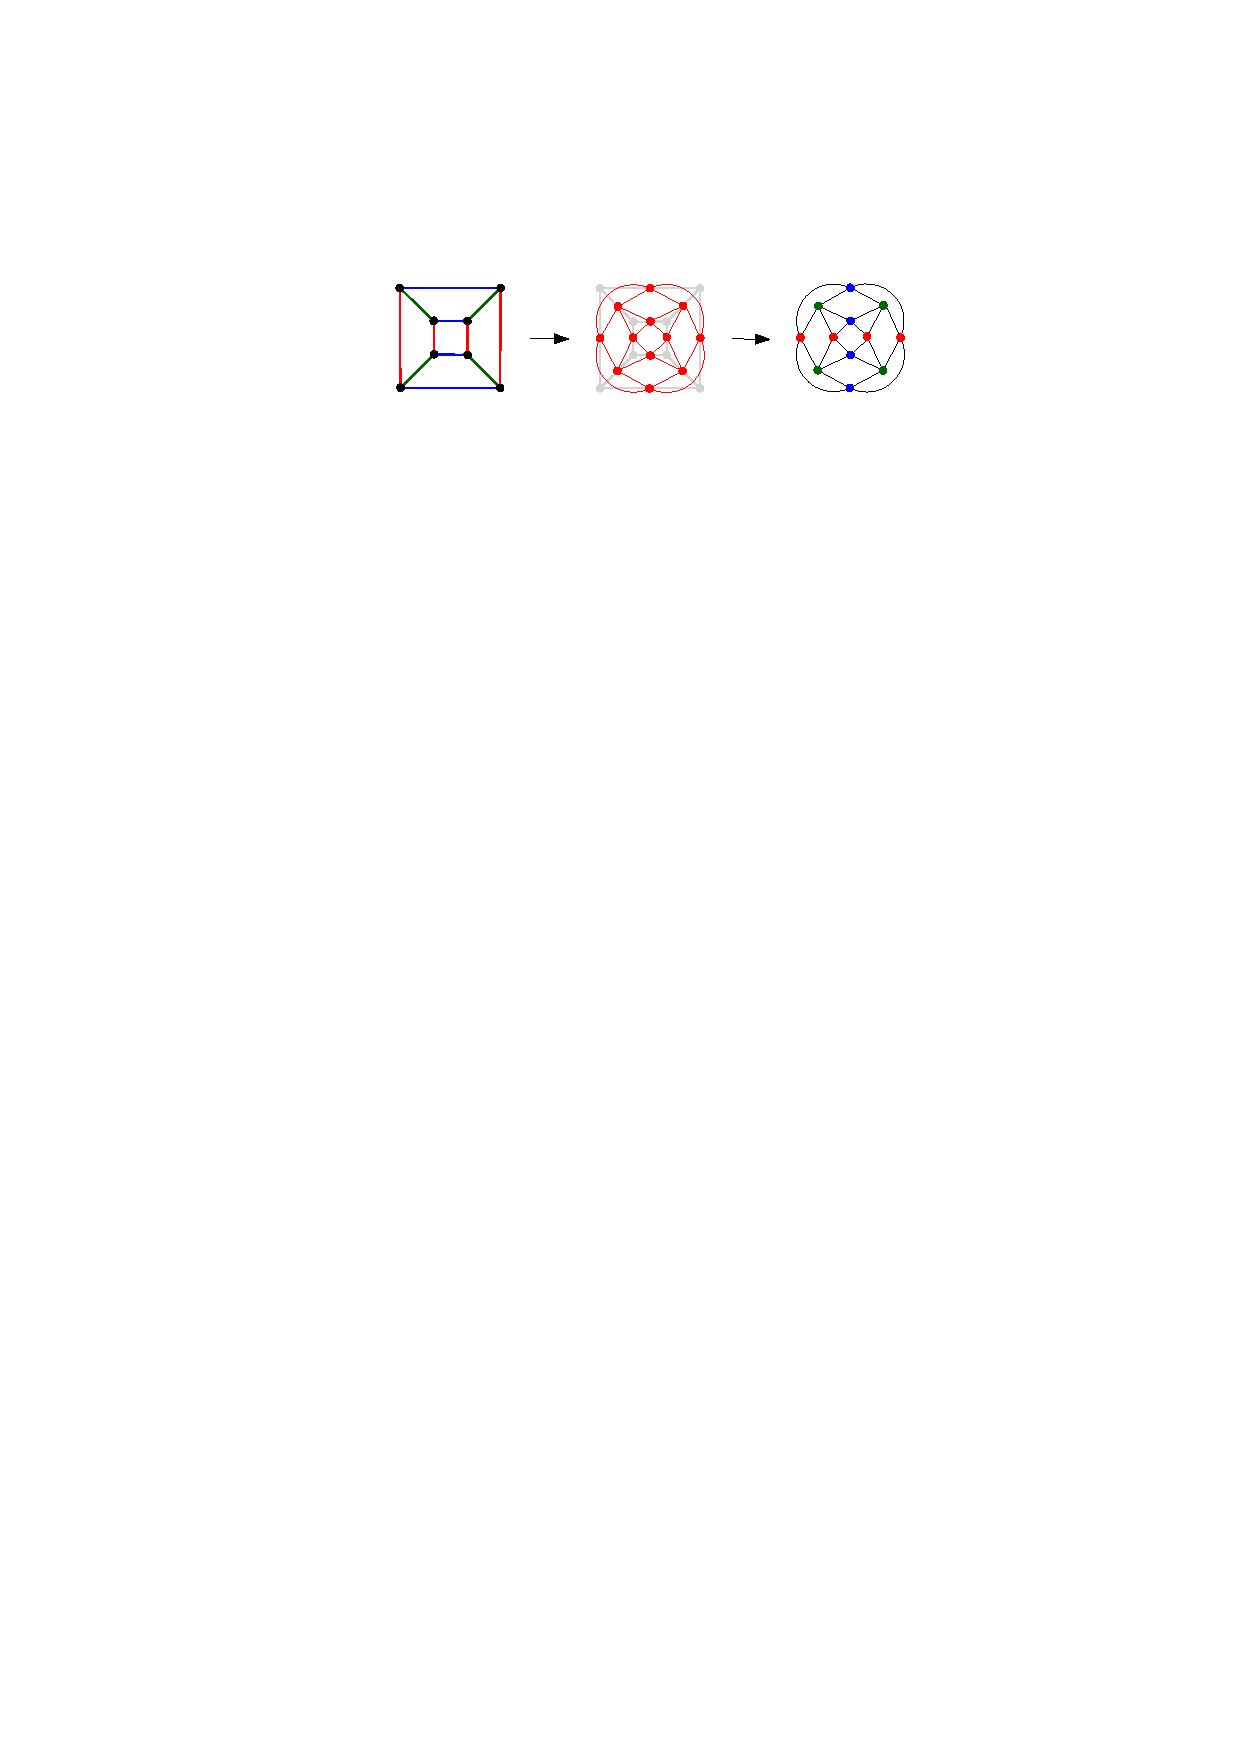
\includegraphics[width=1\textwidth]{../Resources/Figs/cubical_line_graph.pdf}
    \caption{Visualisation of conversion from edge coloring to vertex coloring using a line graph}
    \label{fig:cubical_line_graph}
\end{figure}

Note that in the figure \ref{fig:cubical_line_graph} above, the operation of creating the line graph corresponds to the cube rectification operation. This took us from the graph of a cube to the graph of a cuboctahedron.

\vspace{5pt}
\todo[inline]{TODO: Elaborate more on why creating a line graph from 3-regular graph corresponds to the truncation operation}

\section{Total coloring to vertex coloring}

Intuitively, since total coloring assigns colors to both edges and the vertices, it makes sense that we will use a combination of the original graph with its line graph. Also, we can see, that we cannot just simply take these two graphs and apply vertex coloring on the resulting graph. The problem being, that we would lose the information about what vertex was incident with what edge. This brings us to a so called \textit{incidence graph}.

\begin{definition}[incidence graph]
    For a graph $G=(V,E)$ we define its \emph{incidence graph} $G_I=(V_I,E_I)$ as follows:
    \begin{enumerate}
        \item $V_I := V \cup E$
        \item $E_I = \{\{v,e\} : v \in V, e \in E, v \in e \}$
    \end{enumerate}
\end{definition}

Again, note how the definition of $E_I$ corresponds to the coloring rule \ref{eqn:tot_rule}.

\begin{figure}[H]
    \centering
    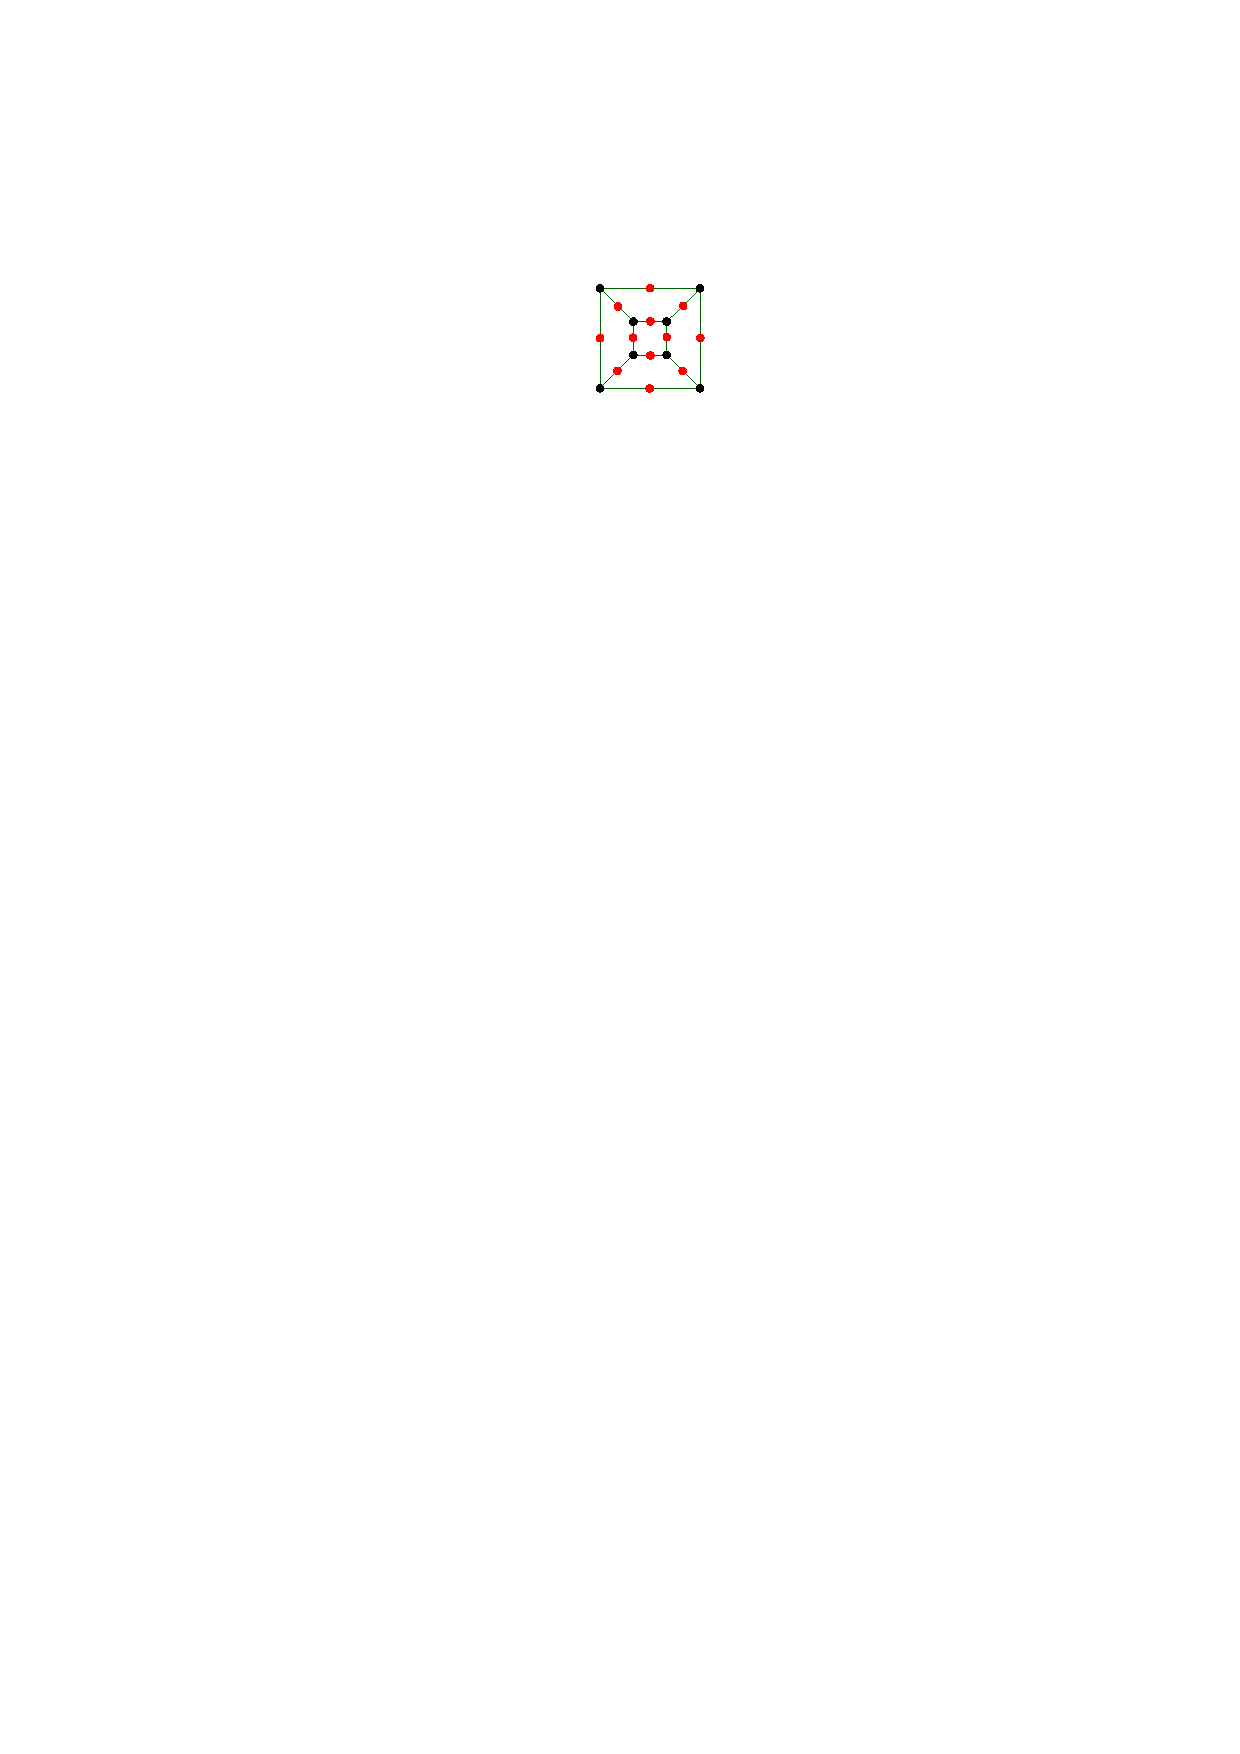
\includegraphics[width=0.2\textwidth]{../Resources/Figs/cubical_incid_graph.pdf}
    \caption{Example of incidence graph of a cubical graph}
    \label{fig:cubical_incid_graph}
\end{figure}

Now we have all the necessary tools to define a \textit{total graph} which will have the property, that its vertex coloring corresponds exactly to total coloring of the original graph.

\begin{definition}[total graph]
    Let $G=(V,E)$ be a graph. Let $G_L =(V_L,E_L)$ and $G_I=(V_I,E_I)$ be its line graph and incidence graphs respectively. We define its \emph{total graph} $G_T=(V_T,E_T)$ as follows:
    \begin{enumerate}
        \item $V_T := V_I$
        \item $E_T := E \cup E_L \cup E_I$
    \end{enumerate}
\end{definition}

In natural language, what we do is, that we start with the vertices and edges of the incidence graph. Then we add the edges of original graph between the vertices that correspond to the original graph. Lastly we interconnect the vertices corresponding to the line graph vertices with the edges of the line graph.

\begin{figure}[H]
    \centering
    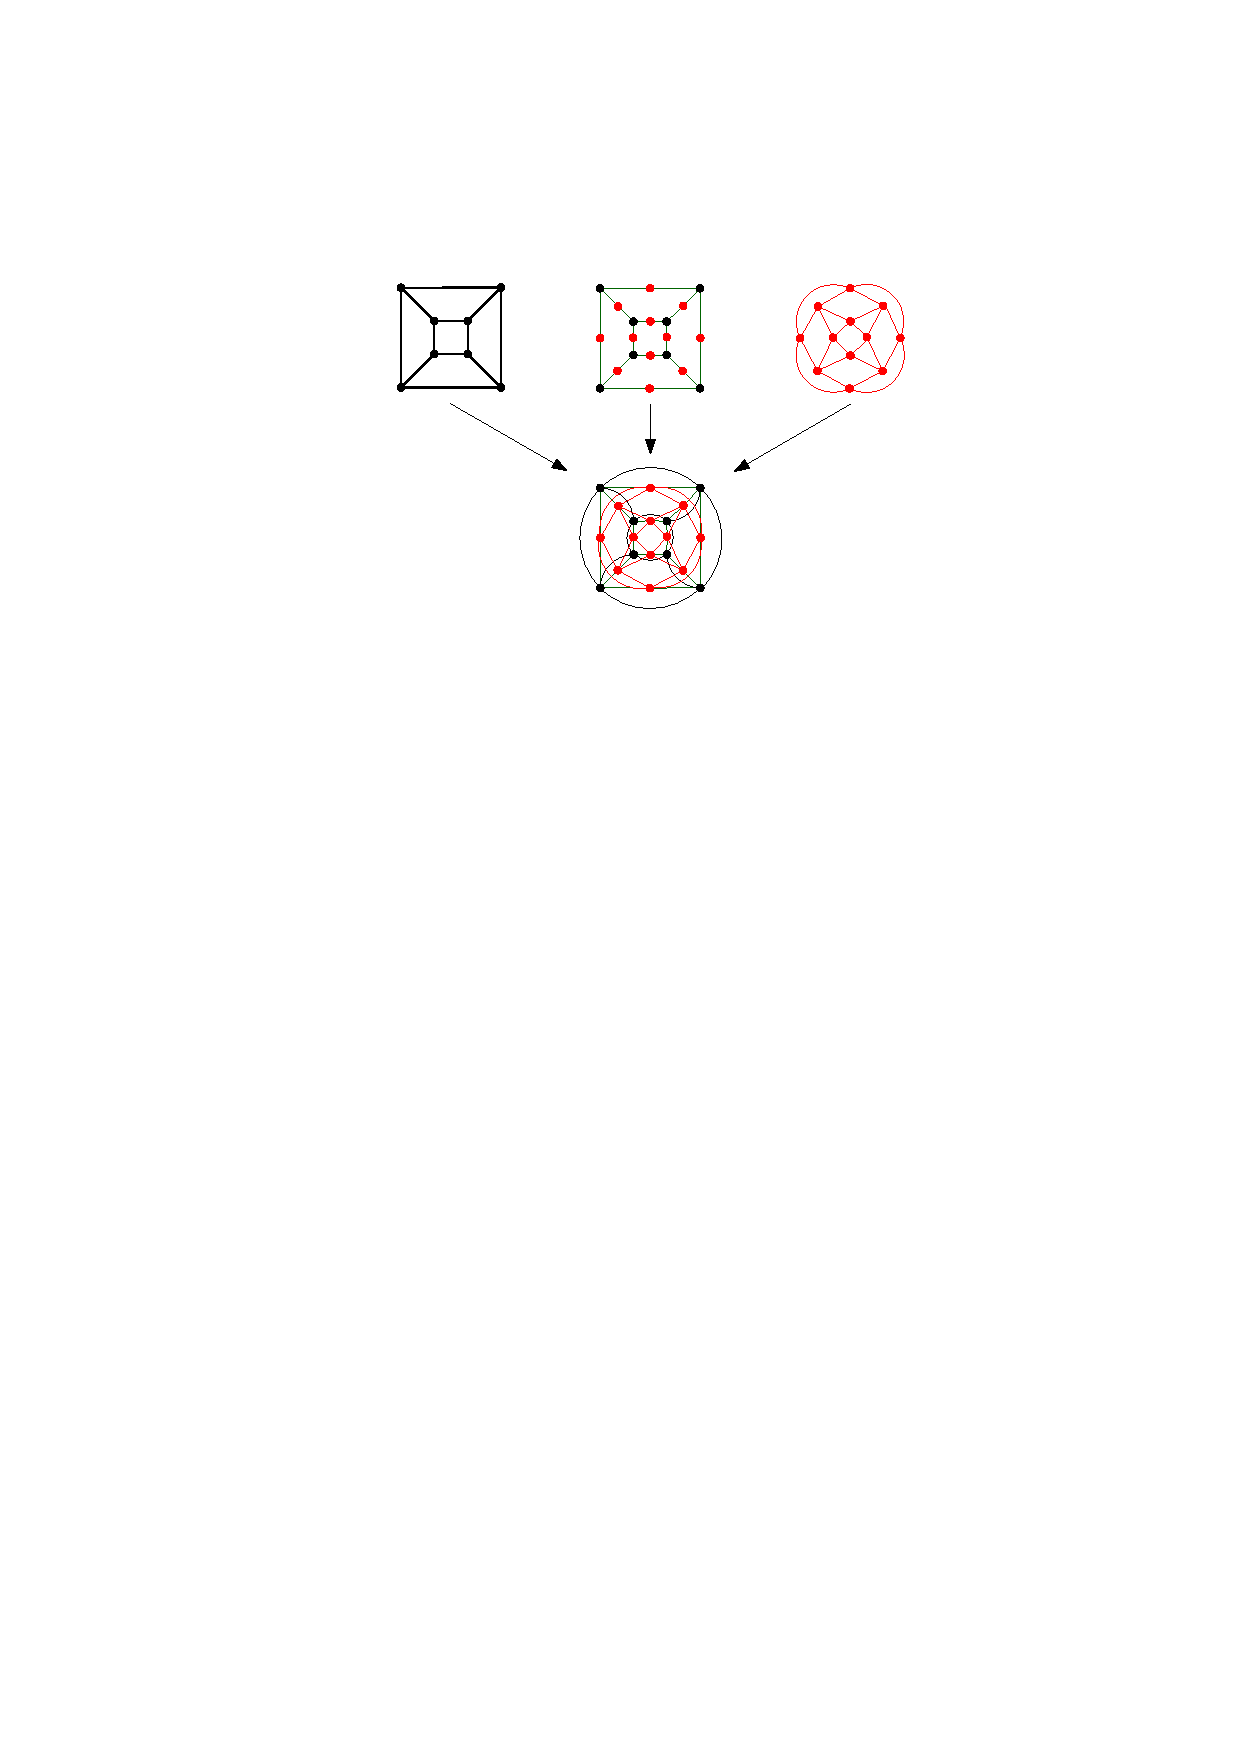
\includegraphics[width=1\textwidth]{../Resources/Figs/cubical_total_graph.pdf}
    \caption{Visualisation of total graph construction from the original graph, incidence graph and line graph respectively.}
    \label{fig:cubical_total_graph}
\end{figure}

\begin{figure}[H]
    \centering
    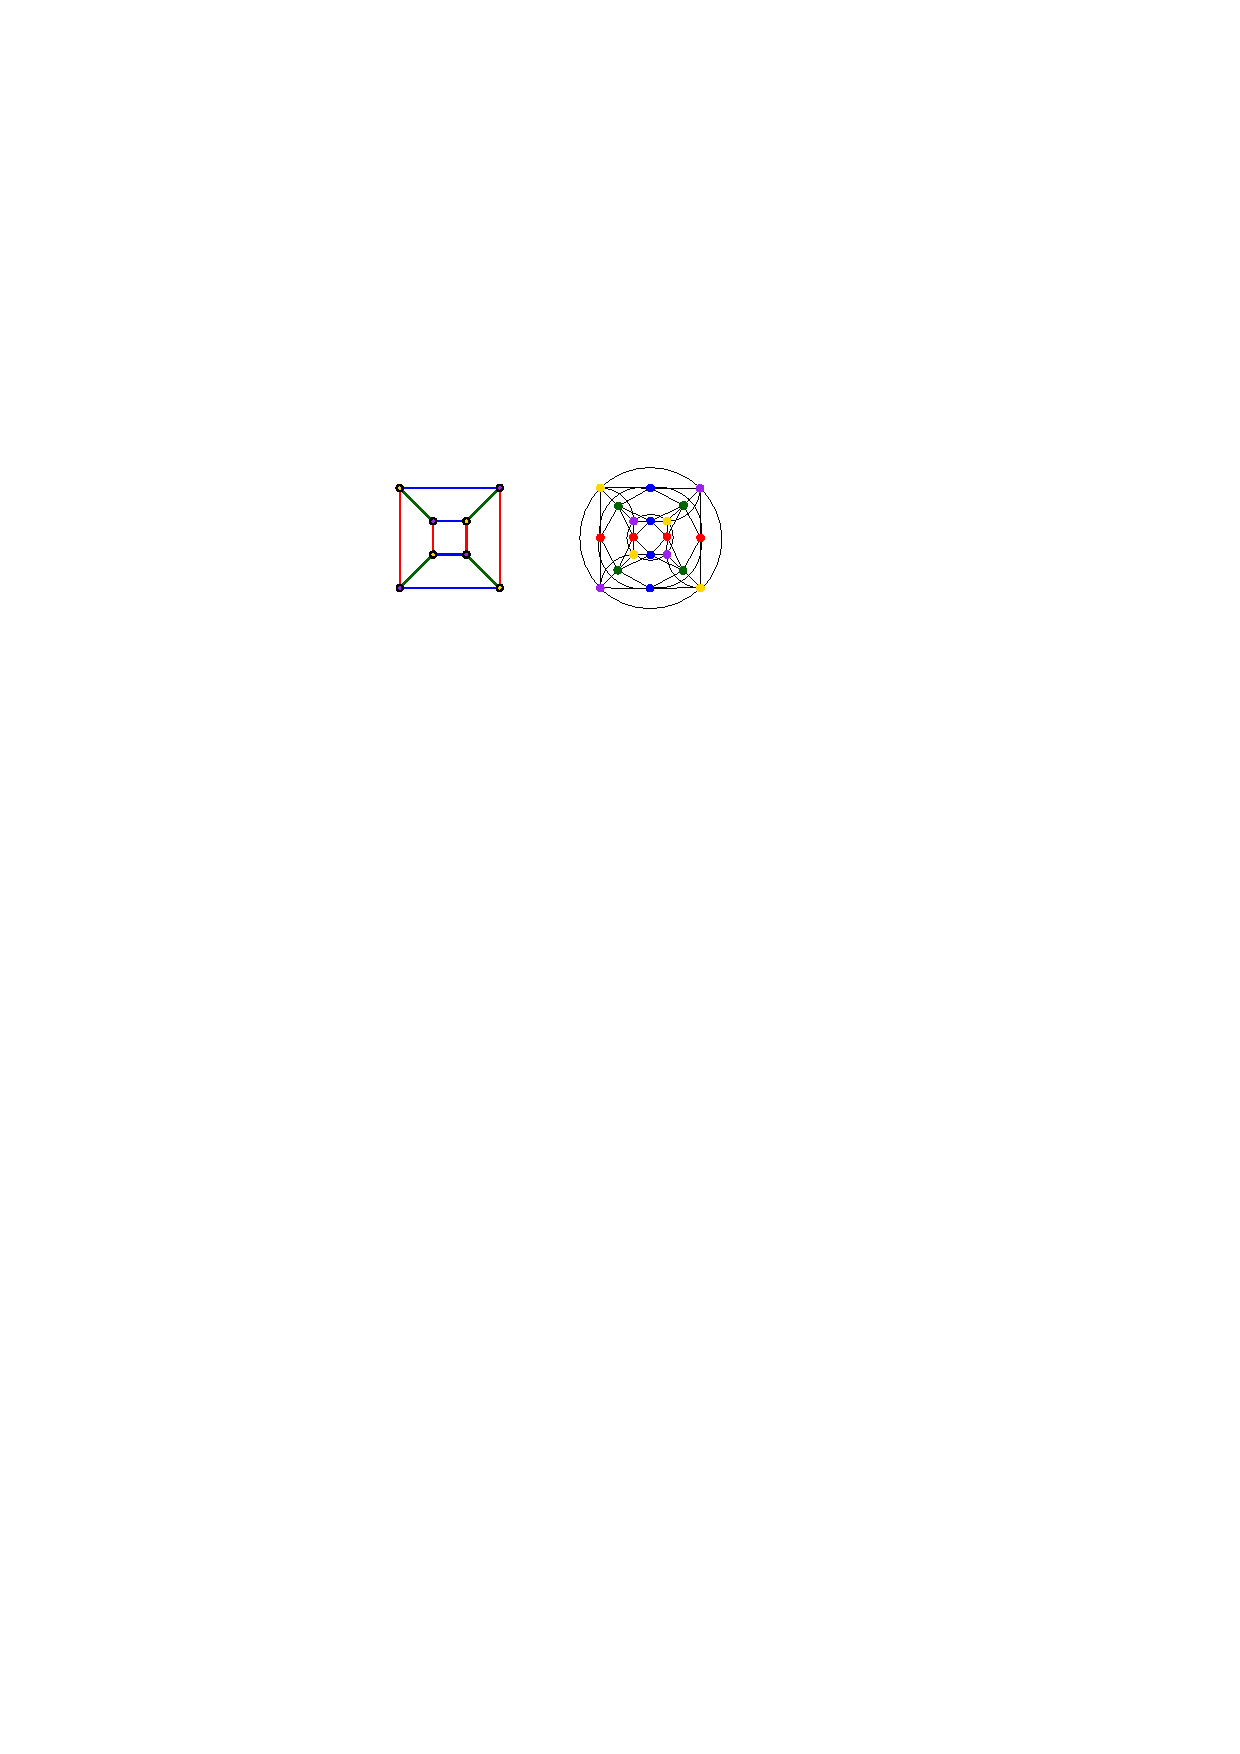
\includegraphics[width=0.6\textwidth]{../Resources/Figs/cubical_tot_g_clring.pdf}
    \caption{Correspondence between total coloring of original graph and vertex coloring of its total graph.}
    \label{fig:cubical_tot_g_clring}
\end{figure}

\section{Face coloring to vertex coloring}

For conversion from face coloring to vertex coloring, we apply the same idea as we did when constructing line graphs. But since the elements colored are faces and not edges, we need to encode incidence of faces into the new graph by adding new edges where necessary. The resulting graph is called a \textit{dual graph}.

\begin{definition}[dual graph]
    For a plane graph $G=(V,E,F)$ we define its \emph{dual graph} $G_D=(V_D,E_D)$ as follows:
    \begin{enumerate}
        \item $V_D := F$
        \item $E_D := \{ \{R_1,R_2\} \in \binom{F}{2}: \bnd(R_1) \cap \bnd(R_2) \neq \emptyset \}$
    \end{enumerate}
\end{definition}

\begin{figure}[H]
    \centering
    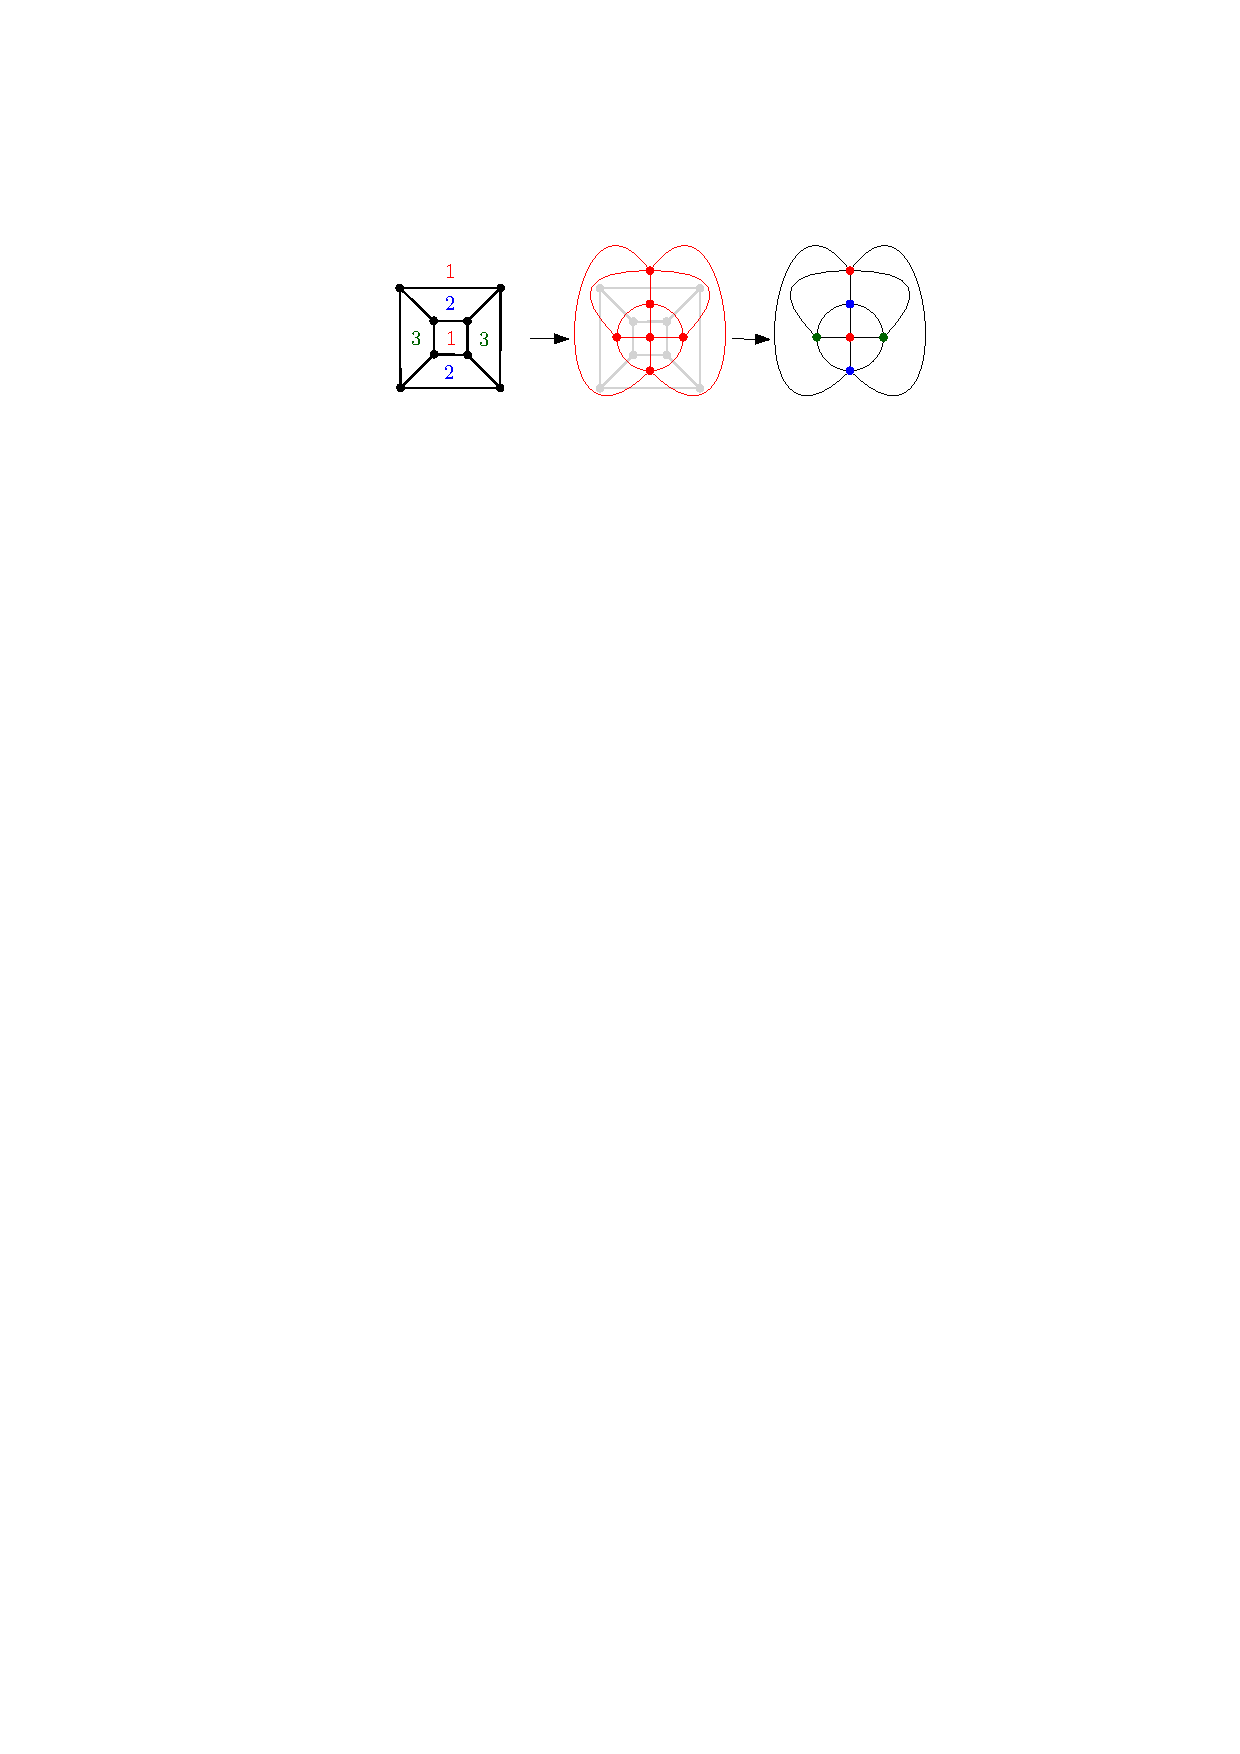
\includegraphics[width=1\textwidth]{../Resources/Figs/cubical_dual_graph.pdf}
    \caption{Visualisation of conversion from face coloring to vertex coloring using a dual graph}
    \label{fig:cubical_dual_graph}
\end{figure}